\chapter{Implementation}
This chapter will discuss the process in which the application was created and will look at each individual step within this process. There are 4 main areas to be discussed. Firstly, generating a basic 3D world, then building on this to produce a representation of the state which allows user interaction. The next task, which is independent to the first, would be to produce the SHA-3 algorithm. It will then look at producing the specific tools for the application, as previously mentioned in chapter 3. Finally, it will look at implementing the user interface, with the navigation keys and menu.
\vspace{5mm}\\
The reason for breaking a large project down into stages, is to allow each stage to be tested individually and to allow for any bugs to be caught early on in the development. Therefore isolating the bug to a specific area and making the solution of any problems much simpler. Although when developing like this it does introduce new problems such as compatibility. Therefore, ensuring that when developing two individual systems, which are to be merged later, it is important that the same format for shared data is used, making merging the systems much easier.
\vspace{5mm}\\
\textit{All of the objects and Java3D terminology in this chapter will be discussed in the level of detailed required to gain a good understanding, but for more information visit the Java3D documentation page\cite{Java3dDoc}.}
\vspace{10mm}\\
\section{3D World}
Developing a 3D world, containing a visual representation of a state, is the foundation of this application, meaning this is the best place to start developing the application. The first task is to develop a ``universe'', using the Java3D library . A ``universe'' contains the canvas, which is where all the 3D objects are drawn. 
\vspace{5mm}\\
The CreateCubes class is where the 3D world is produced. It uses predefined static variables to set the width, depth and height of each cube in the state, where as the users initial view of the state varies, and is calculated, dependant upon the size of the state in use. This is to ensure a better user experience when dealing with larger states.
\vspace{5mm}\\
Directional lighting is produced within this class, to give the user a sense of depth when visualising the state. The lighting is implemented such that the light souce appears to be just off screen. The positioning of the lighting is set with a 3D vector, vector3f, and the correct positioning is essential to making the viewing of the state ease on the eye.
\vspace{5mm}\\
The class also holds two 3-dimensional arrays. The first, ``cubes'', is used to control the cubes which are used to visualise state. Each element stores a single cube, with the appearance of that cubes also kept alongside it, making it vary easy to change the colour, shading and lighting of each cube. The second array, ``currentState'', stores the current values of the state. The values stored in this array is dependant on what the visualisation is required to show. For example, if the state was required to display SHA-3 then the values stored will be either a 1 or 0.
\vspace{5mm}\\
 Each 3D array is indexed such that access the same point in each array refers to the same point in the state. This makes updating the cube much easier, as when the values of the state need to be changed, it is simple to also update the cubes appearance at the same time.
\vspace{5mm}\\
Figure \ref{fig:appState} shows the current representation of the state, if populated with random bits, where black cubes represent a bit value of 1 and white cubes represent a bit value of 0.
\begin{figure}[h!]
\centering
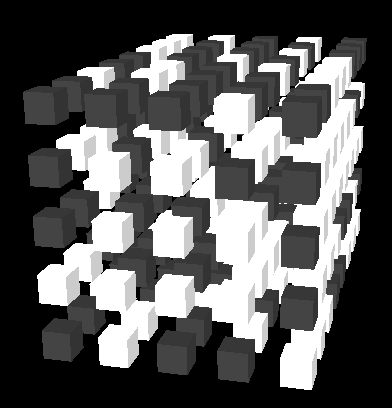
\includegraphics[width=0.5\textwidth]{appState.png}
    \caption{Visual Representation of the State in SHA-3}
    \label{fig:appState}
\end{figure}
\section{SHA-3 Algorithm}
The SHA-3 algorithm is developed in its own class, ``SHA3'', and the class consists of 7 functions
\vspace{5mm}\\
The first 5 functions are the sub-rounds, Theta, Rho, Pi, Chi and Iota. Each take in the 3-dimensional array, the state, with the exception of Iota, which also takes in an integer, the current round. The output of each function is the state, returned in the same format as it was input, a 3-dimensional array.
\vspace{5mm}\\
After completing each of the sub-rounds, it becomes very simple to produce the 6th function, a complete single round of SHA-3, by simple running each sub-round sequentially in succession. Then repeating each round the required number of times, 24 for the complete SHA-3 algorithm, produces a complete algorithm. The complete SHA-3 function can be seen in figure \ref{fig:completeSHA-3}.
\begin{figure}[h!]
\centering
\begin{lstlisting}
SHA3(int[][][] state) {
  for (int i = 0; i < rounds ; i++) {
    state = theta(state);
    state = rho(state);
    state = pi(state);
    state = chi(state);
    state = iota(state, i);
  }
  printHash(state);
};
\end{lstlisting}
\caption{Complete dunction for SHA-3}
\label{fig:completeSHA-3}
\end{figure}
\vspace{5mm}\\
The final function takes in a state as input and outputs a string. This function represents the final stage of SHA-3, returning a hexadecimal string, the hashed value, of the input.
\subsubsection{Problems}
When producing the algorithm in the Java programming language, taking an implementation of the algorithm already produced in not a possibility. As previously mentioned, other implementations merge the sub-rounds together into one concise function.
\vspace{5mm}\\
Alongside the aforementioned issue, other implementation can sometimes be difficult to understand what is occuring in each of the sub-round functions. Functions which allow for an easier understand could also be used in the explanation of SHA-3 and be much more beneficial to the student/tutor. Both of these points are easily demonstrated in figure \ref{fig:RhoPi}.
\begin{figure}[h!]
\advance\leftskip-2cm
\begin{subfigure}{.6\textwidth}
    \begin{lstlisting}
rho(int[][][] state) {
  int newState[stateWidth]
    [stateHeight][stateDepth];
  for(x=0; x<stateWidth; x++) {
    for(y=0; y<stateHeight; y++) {
      for(z=0; z<stateDepth; z++) {
        newZ = (z +
          rotation_const[x][y])
          % stateDepth;
        newState[x][y][newZ]
          = state[x][y][z];
      }
    }
  }
  return newState;
};
    \end{lstlisting}
    \caption{Application's Implementation of $\rho$ \emph{in Pseudocode}}
    \label{fig:sub1RhoP}
\end{subfigure}
\advance\rightskip-2cm
\hfill\begin{subfigure}{.6\textwidth}
    \begin{lstlisting}
pi(int[][][] state) {
  int newState [stateWidth]
    [stateHeight][stateDepth];
  for( x=0; x<stateWidth; x++) {
    for( y=0; y<stateHeight; y++) {
      for ( z=0; z<stateDepth; z++) {
        newX = y;
        newY = (2 * x + 3 * y)
          % stateHeight;
        newState[newX][newY][z]
          = state[x][y][z];
      }
    }
  }
  return newState;
};
    \end{lstlisting}
    \caption{Application's Implementation of $\pi$ \emph{in Pseudocode}}
    \label{fig:sub2RhoPi}
\end{subfigure}
\begin{center}
\begin{subfigure}{.6\textwidth}
\centering
\begin{lstlisting}
temp = state[1];
for (x=0; x<24; x++){
  BC[0] = state[KeccakF_PiLane[x]];
  state[KeccakF_PiLane[x]] = ROL(temp,
    KeccakF_RotationConstants[x]);
  temp = BC[0];
}
    \end{lstlisting}
    \caption{Keccak's Implementation of both $\pi$ and $\rho$ \emph{in C}}
    \label{fig:sub3RhoP}
\end{subfigure}
\end{center}
\caption{SHA-3 Sub-rounds $\rho$ and $\pi$}
\label{fig:RhoPi}
\end{figure}
\vspace{5mm}\\
Understandable in doing this efficiency and neatness is compromised, but these are not the main aims of the project therefore they are a necessary compromise. 
\vspace{5mm}\\
The Keccak website\cite{KeccakSite} and the SHA-3 wikipedia page\cite{SHA3Wiki} both have documentation which give a broken down implementation of SHA-3. Using this documentation, each subround was re-created in turn, in it's most simple form for understanding and seperating out each sub-round in turn.
\vspace{0mm}\\
\textit{It must be noted that while the Keccak website and the SHA-3 wikipedia page provide extremely useful information, they do contain conflicts in notation and one must be careful when using multiple sources to check for any conflicts and avoid confusion.}
\section{Tools}
This section will look at the implementation of each of the tools mentioned in the previous chapter.
\subsection{Visualising SHA-3}
After completing the visualisation of the state and the SHA-3 algorithm, the next stap would be to merge the two implementations to give one working system.
\vspace{5mm}\\
From acknowledging a future problem, the compatibility of the two components, early on in the implementation, it has made the process of merging the two separate parts into one much easier. This is because the creation of the state in the CreateCubes class is of the same format which is too be entered into SHA-3 and also the same output of SHA-3. This means when the state is randomly generated, it can be immediately passed to the SHA-3 algorithm before an array of states being returned, with each element containing the state at each point in the algorithm. Now any element in this array can be selected and displayed using the CreateCubes class, showing how the state progresses throughout SHA-3.
\subsection{Sub-Rounds}
First Paragraph
\vspace{5mm}\\
Second Paragraph
\subsection{Cumulative Difference}
First Paragraph
\vspace{5mm}\\
\begin{figure}[h!]
\advance\leftskip-2cm
\begin{subfigure}{.6\textwidth}
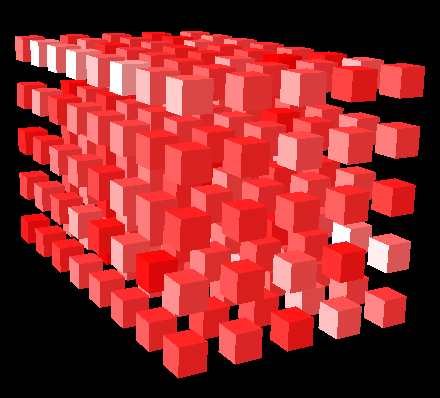
\includegraphics[width=1\textwidth]{CummulativeDifference.png}
    \caption{Visual Representation of the State in SHA-3}
    \label{fig:appState}
\end{subfigure}
\advance\rightskip-2cm
\hfill\begin{subfigure}{.6\textwidth}
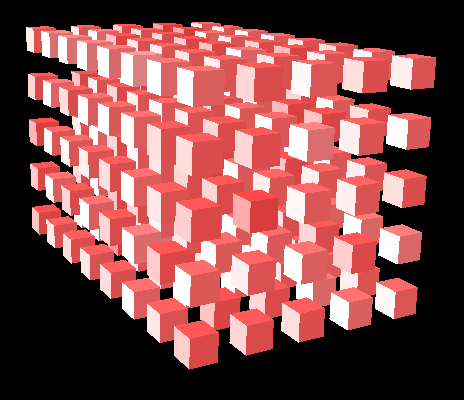
\includegraphics[width=1.048\textwidth]{CummulativeDifferenceEarly.png}
    \caption{Visual Representation of the State in SHA-3}
    \label{fig:appState}
\end{subfigure}
\caption{SHA-3 Sub-rounds $\rho$ and $\pi$}
\label{fig:CummulativeDifference}
\end{figure}
\vspace{5mm}\\
\subsection{Random Bit Difference}
First Paragraph
\vspace{5mm}\\
Second Paragraph
\subsection{Random Bit Difference Summation}
First Paragraph
\vspace{5mm}\\
Second Paragraph
\subsection{Navigation Bar and Menu}
First Paragraph
\vspace{5mm}\\
Second Paragraph